% 正态分布概率密度函数,\sigma参数的变化情况
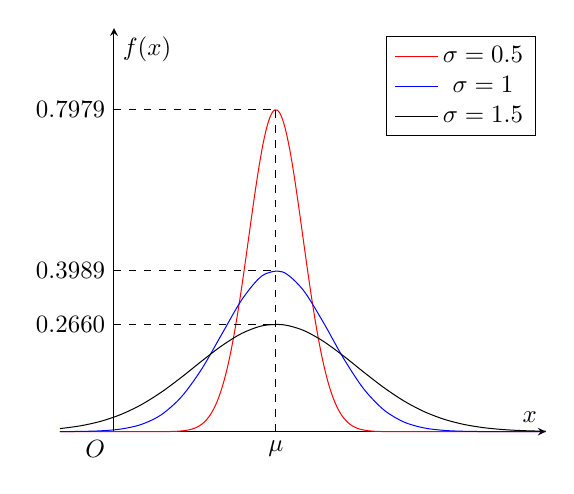
\begin{tikzpicture}[scale = 0.9]
  \begin{axis}[clip=false,xmin=-1, xmax=8,ymin=0,ymax=1, axis lines = middle,
    smooth, xlabel={$x$}, ylabel={$f(x)$},ticks=none]
    % mu = 3, sigma = 0.5
    \addplot[draw=red,domain=-1:8,samples=200] {0.7979 * e^(-((x-3)^2)/0.5)};
    % mu = 3, sigma = 1
    \addplot[draw=blue,domain=-1:8] {0.3989 * e^(-((x-3)^2)/2)};
    % mu = 3, sigma = 1.5
    \addplot[draw=black,domain=-1:8] {0.2660 * e^(-((x-3)^2)/4.5)};

    % y = 0.7979, [0,3],最高点
    \draw[dashed] (0,0.7979) -- (3,0.7979);
    \node[left] at (0,0.7979) {$0.7979$};
    % y = 0.3989, [0,3],最高点
    \draw[dashed] (0,0.3989) -- (3,0.3989);
    \node[left] at (0,0.3989) {$0.3989$};
    % y = 0.2660, [0,3],最高点
    \draw[dashed] (0,0.2660) -- (3,0.2660);
    \node[left] at (0,0.2660) {$0.2660$};

    \draw[dashed] (3,0) -- (3,0.7978);
    \node[below] at (3,0) {$\mu$};

    % 原点标签
    \node[below left] at (0,0) {$O$};

    % 图示
    \addlegendentry{$\sigma=0.5$}
    \addlegendentry{$\sigma=1$}
    \addlegendentry{$\sigma=1.5$}
  \end{axis}
\end{tikzpicture}
